\documentclass[11pt,a4paper]{ivoa}
\usepackage[margin=4.25cm]{geometry}
\usepackage{array}
\usepackage{lscape}
\usepackage{longtable}
\input tthdefs
\setcounter{tocdepth}{2}

\title{Dataset Metadata Model}

% see ivoatexDoc for what group names to use here
\ivoagroup{Data Model Working Group}

%\author[????URL????]{????Alfred Usher Thor????}
\author{Mark Cresitello-Dittmar, Francois Bonnarel, Omar Laurino, Gerard Lemson, Mireille Louys, Arnold Rots, Doug Tody}

\editor{Mark Cresitello-Dittmar}

% \previousversion[????URL????]{????Funny Label????}
\previousversion[https://www.ivoa.net/documents/DatasetDM/20170928/WD-DatasetDM-1.0-20170928.pdf]{WD-DatasetDM-1.0-20170928}


\begin{document}

\begin{abstract}
  This document provides a data model describing the structure and content of
  generic Dataset metadata for the IVOA. This is a high-level model which is
  to be referenced and extended by other models describing specific types of
  Datasets and Data products. In this document, we specify the generic Dataset,
  as well as an ObservationDataset model which covers the class of Datasets
  which are derived from an Observation. At the time of this writing, there
  is no formal Observation-Experiment model for the IVOA, so we include a
  hypothetical Observation-Experiment model to serve as a placeholder.
\end{abstract}

% Table of Contents goes here. (auto)
% List of Figures goes here.
\listoffigures

\section*{Acknowledgments}
TBD

\section*{Conformance-related definitions}
The words ``MUST'', ``SHALL'', ``SHOULD'', ``MAY'', ``RECOMMENDED'', and
``OPTIONAL'' (in upper or lower case) used in this document are to be
interpreted as described in IETF standard RFC2119 \citep{std:RFC2119}.

The \emph{Virtual Observatory (VO)} is a general term for a collection of
federated resources that can be used to conduct astronomical research, education, and outreach.
The \href{http://www.ivoa.net}{International Virtual Observatory Alliance (IVOA)}
is a global collaboration of separately funded projects to develop standards and
infrastructure that enable VO applications.



\newgeometry{left=1.0in,right=1.0in,bottom=1.0in}
\section{Introduction}

\subsection{Motivation}
All IVOA datasets must contain a common set of metadata elements to facilitate
the registration, discovery, and interoperability of these datasets. To date,
individual IVOA data models have independently defined this metadata within
the separate documents. This has resulted in some level of inconsistency between
models, as well as document bloat, and some ambiguity as to the hierarchy and
relation of models to each other. For example, the ObsCore-1.0 model describes
itself as defining "the core components of the Observation data model ", but
there is no formal definition of an Observation data model in the IVOA. Without
this higher-level document, it is difficult for detailed models to properly
reference and/or extend this content consistently.

With the development of the Cube model, significant effort has been made to
properly model this high-level metadata, and separate the components related
to the generic dataset, a dataset derived from an observation, and the
observation itself. This document represents the results of that effort. Here,
we define the generic dataset metadata, and provide an example for extending
this with metadata related to datasets resulting from a specific process
(Observation). As such, the ObsCore model should be considered a 'view' of this
model, highlighting the core components required for supporting TAP services.

The descriptions of many elements of this model are a result of reviewing and
combining those contained in the ObsCore (1.0) \citep{2011ivoa.spec.1028T}, Spectrum (1.1) \citep{2011ivoa.spec.1120M}, and
Characterisation (1.13) \citep{2008ivoa.spec.0325L} models.
As such, it represents a uniform, consistent
description set. Future revisions of those documents should be defined with
respect to this model.

%\subsection{Context and Scope}
%
%\section{Use Cases and Requirements}
%\label{sect:ucreq}
%
%\subsection{Use Cases}
%\label{sect:usecases}
%
\subsection{Requirements}
\label{sect:reqs}

The primary goals of this document are:
\begin{itemize}
  \item to provide a specification of generic dataset metadata sufficient to
    support current IVOA data product models and access protocols.
  \item to specify metadata associated with an Observation (experiment) which are
    to be included in datasets derived from observations (ObsDataset).
\end{itemize}    

%\subsubsection{General}
%
%\subsubsection{Application/Usage}
%
%\subsubsection{Content}

\pagebreak
\subsection{Role within the VO Architecture}

\begin{figure}[h]
\centering

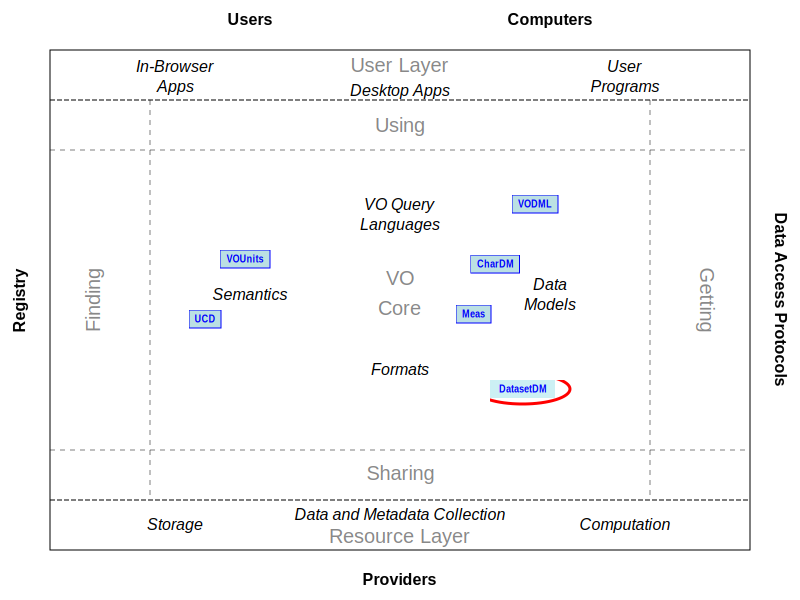
\includegraphics[width=0.9\textwidth]{role_diagram.pdf}
\caption{Architecture diagram for this document}
\label{fig:archdiag}
\end{figure}

%Fig.~\ref{fig:archdiag} shows the role this document plays within the IVOA architecture \citep{2010ivoa.rept.1123A}.


\pagebreak
\subsection{Model Dependencies}

\begin{figure}[h]
\centering

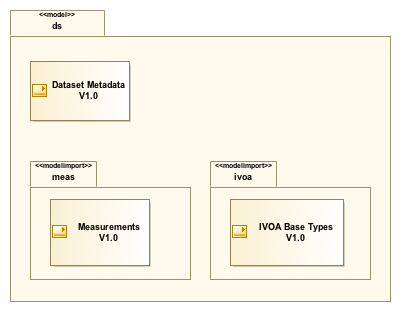
\includegraphics[width=0.6\textwidth]{diagrams/model_dependencies.png}
\caption{Model dependency diagram}
\label{fig:dependencies}
\end{figure}

The Dataset model is built on other data models as indicated in Figure \ref{fig:dependencies}.
The <<model>> and <<modelimport>> stereotypes provide information identifying the
model, it's version, any dependencies, and URLs to find more information about
the model definitions including HTML and schema documentation. See Appendix \ref{sect:stereotypes}
for more information about the content of these stereotypes and how they are
used in serializations.

\subsection{Structure of this Documentation}
\begin{itemize}
  \item  Major sections for each model area (Dataset, Observation, etc. ).
  \item  First subsection in each section is the primary element within that model
  \item  Subsequent subsections for secondary elements, generally in alphabetical order,
but occasionally a logical grouping of related objects makes more sense.
  \item  Each subsection has sub-subsections for each attribute/relation
  \begin{itemize}
    \item  attributes show the full definition including datatype and usage.
    \item  relations describe the usage of the object in that context,
      the type of the target of the relation, and a reference to the full
      definition of that type.
  \end{itemize}
  \item  Capitalization convention
  \begin{itemize}
    \item  Objects and complex data types are expressed in PascalCase
    \item  Attributes are camelCase
    \item  Primitive data types (string, double, etc.) are lower case
  \end{itemize}
\end{itemize}


% Main Body of the document
\pagebreak
% --------------------------------------------------------------------------------
%                                  Dataset Model
% --------------------------------------------------------------------------------
\section{Dataset Model}
\label{sect:ds}

This section describes the generic, high-level metadata associated with an
IVOA Dataset. Since serialization format choices may effect the number of
files or components which comprise a dataset, we define an IVOA Dataset as
"a file or files which are considered to be a single deliverable".
Examples of viable datasets include:
\begin{itemize}
  \item An individual data product, such as a Spectrum, or Image.
  \item A 'tar' file or directory of processed observational data files.
\end{itemize}

This metadata identifies the dataset, and provides information regarding the
ownership, rights and associations with other datasets. The primary purpose
of this metadata is to facilitate the registry and discovery of datasets
within the IVOA community.

Several of the objects modeled here are based on descriptions given in the IVOA
document, "Resource Metadata for the Virtual Observatory; Version 1.12" \citep{2007ivoa.spec.0302H}
(Resource Metadata). Where applicable, we provide the appropriate citation
in the text below.

% INSERT FIGURE HERE
\begin{figure}[h]
\begin{center}
  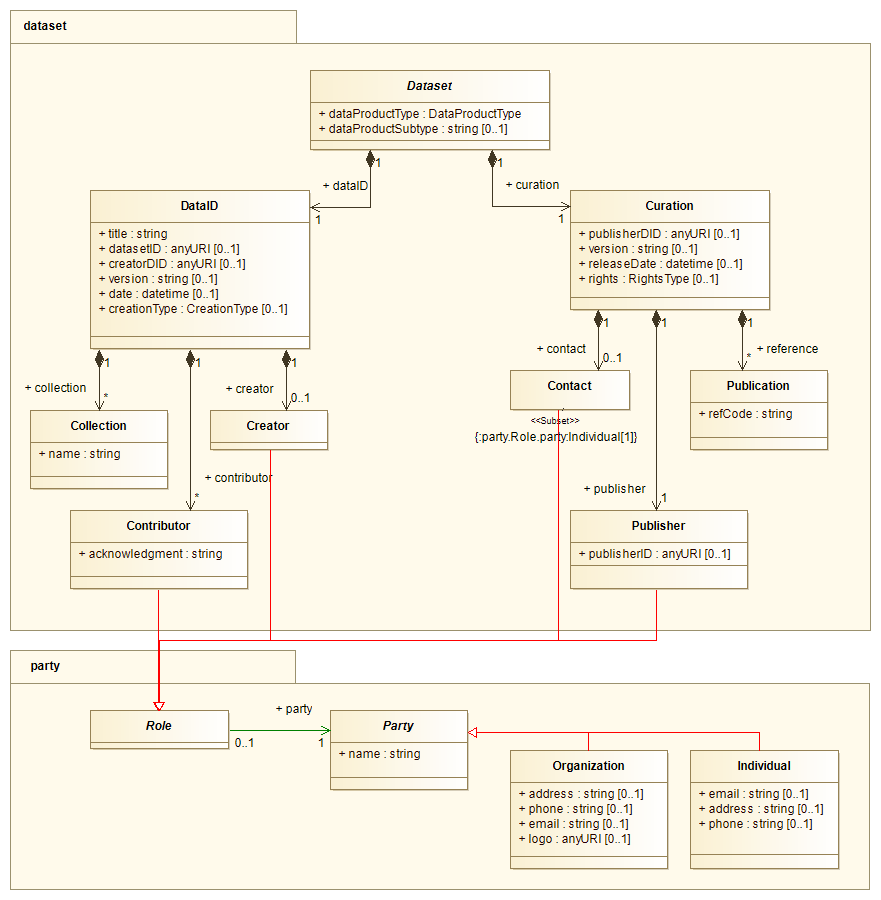
\includegraphics[width=5.0in]{diagrams/Dataset_overview.png}
  \caption{Generic Dataset Metadata}\label{fig:ds_overview}
\end{center}
\end{figure}

\pagebreak
\subsection{Dataset}
\label{sect:dataset}
% ==================

  % INSERT FIGURE HERE
  \begin{figure}[h]
  \begin{center}
    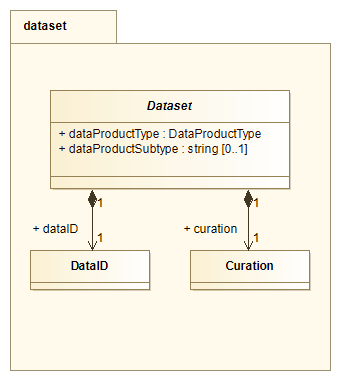
\includegraphics[width=2.5in]{diagrams/Dataset.png}
    \caption{Dataset Metadata detail}\label{fig:ds_detail}
  \end{center}
  \end{figure}

  Abstract object for the generic IVOA Dataset. It is intended to be useful for
  any type of data. Specific dataset models should extend this object, providing
  detailed definitions and additional content as appropriate for that type of dataset.

  \subsubsection{Dataset.dataProductType}
  \textbf{type: \hyperref[sect:product]{DataProductType}} \newline
  \textbf{multiplicity: 1} \newline 
  
  Describes the high level scientific classification of the data content. Values
  are restricted to the DataProductType enumeration set and convey the general
  idea of the content and organization of a dataset.
  
  \subsubsection{Dataset.dataProductSubtype}
  \textbf{type: \hyperref[sect:ivoa]{string}} \newline
  \textbf{multiplicity: 0..1} \newline 

  Secondary type classification for the dataset. This field is intended to
  precisely specify the scientific nature of the data product, possibly in
  terms relevant only to a specific archive or data collection. For example,
  dataProductType='image' could have associated dataProductSubtype="src.image",
  "bkg.image", "PixelMask", etc. Values are unrestricted strings.
  
  \subsubsection{Dataset.curation}
  \textbf{type: \hyperref[sect:curation]{Curation}} \newline
  \textbf{multiplicity: 1} \newline 

  Provides metadata related to the entity responsible for the curation of the dataset.
  
  \subsubsection{Dataset.dataID}
  \textbf{type: \hyperref[sect:dataid]{DataID}} \newline
  \textbf{multiplicity: 1} \newline 

  DataID provides high level identification metadata for the dataset itself, and
  any associations with various collections.  
  
  
\pagebreak
\subsection{Collection}
\label{sect:collection}
% ==================

  % INSERT FIGURE HERE
  \begin{figure}[h]
  \begin{center}
    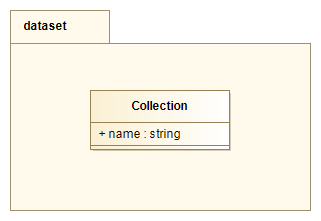
\includegraphics[width=2.25in]{diagrams/Collection.png}
    \caption{Collection detail diagram}\label{fig:collection}
  \end{center}
  \end{figure}

  A generic organizational construct which allows Datasets to be associated with
  each other by a set of Collection properties. Datasets tagged with the same
  Collection properies can be assumed to have some degree of compatibility.

  \subsubsection{Collection.name}
  \textbf{type: \hyperref[sect:ivoa]{string}} \newline
  \textbf{multiplicity: 1} \newline 

  The values are generally defined by the creating entity. Examples: "WFC",
  "Sloan", "BFS Spectrograph", "MSX Galactic Plane Survey".

  
\pagebreak
\subsection{Contact}
\label{sect:contact}
% ==================

  % INSERT FIGURE HERE
  \begin{figure}[h]
  \begin{center}
    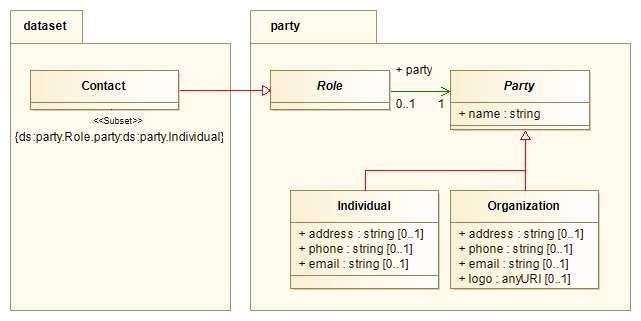
\includegraphics[width=4.75in]{diagrams/Contact.png}
    \caption{Contact detail diagram}\label{fig:contact}
  \end{center}
  \end{figure}

  Contact information for a person or entity.
  
  Contact is modeled as a Role played by a particular person or entity (Party).
  We subset the type of Party to include only Individuals. This includes both a
  physical person, or proxy service such as a helpdesk.
  
  Party package is described in Section \ref{sect:party_pkg}.
  

\pagebreak
\subsection{Contributor}
\label{sect:contributor}
% ======================

  % INSERT FIGURE HERE
  \begin{figure}[h]
  \begin{center}
    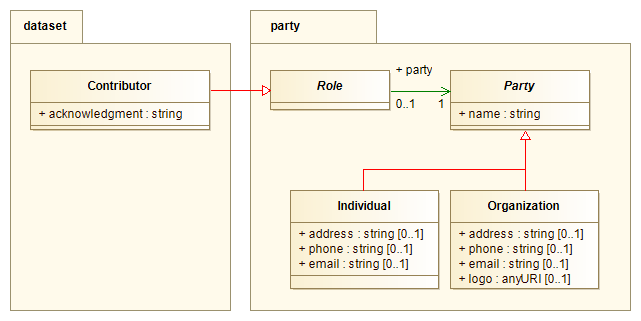
\includegraphics[width=4.75in]{diagrams/Contributor.png}
    \caption{Contributor detail diagram}\label{fig:contributor}
  \end{center}
  \end{figure}

  Contributor is modeled as a Role played by a Party or entity who participated
  in the generation of the Dataset.
  
  Party package is described in Section \ref{sect:party_pkg}.

  \subsubsection{Contributor.acknowledgement}
  \textbf{type: \hyperref[sect:ivoa]{string}} \newline
  \textbf{multiplicity: 1} \newline 

  Acknowledgment expression for the contributor. Users of the dataset should
  include these in subsequent credits and acknowledgements. The expression
  should be formatted as desired by the contributor.
  

\pagebreak
\subsection{Creator}
\label{sect:creator}
% ==================

  % INSERT FIGURE HERE
  \begin{figure}[h]
  \begin{center}
    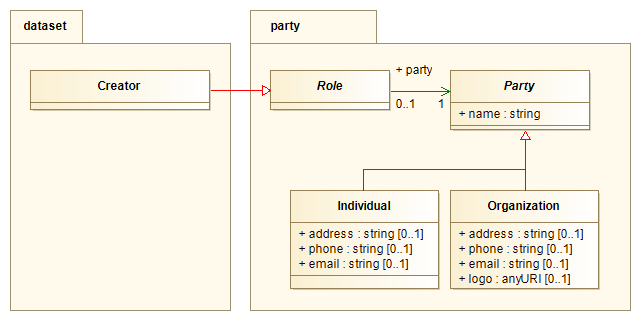
\includegraphics[width=4.75in]{diagrams/Creator.png}
    \caption{Creator detail diagram}\label{fig:creator}
  \end{center}
  \end{figure}

  Creator is modeled as a Role played by the organization or entity which
  created the Dataset.

  Party package is described in Section \ref{sect:party_pkg}.
  
\pagebreak
\subsection{Curation}
\label{sect:curation}
% ==================

  % INSERT FIGURE HERE
  \begin{figure}[h]
  \begin{center}
    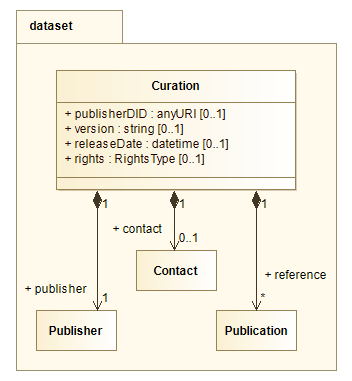
\includegraphics[width=2.375in]{diagrams/Curation.png}
    \caption{Curation detail diagram}\label{fig:curation}
  \end{center}
  \end{figure}

  The Curation object provides metadata assigned by the entity responsible for
  the support of the dataset content as well as identifying metadata about that
  entity. It is assembled from definitions provided by the IVOA Resource
  Metadata document. Here, we provide a brief description of each field for easy
  reference, along with a notation of its mapping to the Resource Metadata
  document (RM:field), where the reader may find more detailed information.

  \subsubsection{Curation.contact}
  \textbf{type: \hyperref[sect:contact]{Contact}} \newline
  \textbf{multiplicity: 0..1} \newline 

  Contact information of the person/entity responsible for the content of the
  dataset. We recommend using a generic 'helpdesk' type contact rather than
  individuals whose information may more easily become obsolete. (RM:Curation.Contact)
  
  \subsubsection{Curation.publisher}
  \textbf{type: \hyperref[sect:publisher]{Publisher}} \newline
  \textbf{multiplicity: 1} \newline
  
  The entity making the data available. (RM:Curation.Publisher)

  \subsubsection{Curation.publisherDID}
  \textbf{type: \hyperref[sect:ivoa]{anyURI}} \newline
  \textbf{multiplicity: 0..1} \newline
  
  IVOA dataset identifier assigned by the publisher to uniquely identify the
  dataset within its holdings. Typically, the basis of this identifier will
  be the publisher ID. However, if the publisher chooses to use a 'global index
  service' such as ADS to obtain persistent identifiers for their datasets,
  rather than generate their own, that identifier should be used both here and
  for DataID.datasetID. Note: this model also defines a creator dataset ID
  (DataID.creatorDID), these will differ if the publishing entity is not
  the creator of the dataset. Values are to be expressed as dataset identifiers
  using the syntax described in "IVOA Identifiers" \citep{2007ivoa.spec.0314P}.
  
  \subsubsection{Curation.reference}
  \textbf{type: \hyperref[sect:publication]{Publication}} \newline
  \textbf{multiplicity: 0..*} \newline
  
  Zero or more bibliographic or documentation references associated with the
  dataset. Each instance provides a single forward link to a major publication
  which references the dataset. (RM:General.Source)
  
  \subsubsection{Curation.releaseDate}
  \textbf{type: \hyperref[sect:dates]{datetime}} \newline
  \textbf{multiplicity: 0..1} \newline
  
  Date the curated dataset was last modified. (RM:Curation.Date)
  
  \subsubsection{Curation.rights}
  \textbf{type: \hyperref[sect:rights]{RightsType}} \newline
  \textbf{multiplicity: 0..1} \newline
  
  Indicates the level of access being granted. Values are restricted to the
  RightsType enumeration set. (RM:Collection.Rights)
  
  \subsubsection{Curation.version}
  \textbf{type: \hyperref[sect:ivoa]{string}} \newline
  \textbf{multiplicity: 0..1} \newline
  
  Version of the curated dataset, assigned by the publisher. This is an
  independent versioning from DataID.version that allows the publisher to track
  changes to the high level dataset metadata (e.g. curation metadata,
  identifiers, etc.) without effecting the creator defined dataset version. The
  value may be based on the DataID.version (e.g. by adding a sub-version extension),
  or an independent versioning. There are no format restrictions on the value. (RM:Curation.Version)  

  
\pagebreak
\subsection{DataID}
\label{sect:dataid}
% ==================

  % INSERT FIGURE HERE
  \begin{figure}[h]
  \begin{center}
    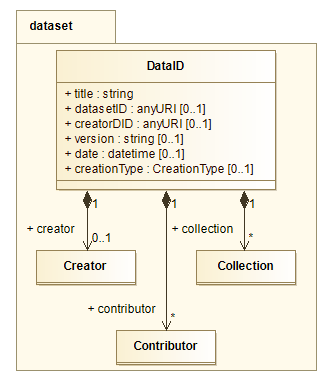
\includegraphics[width=2.375in]{diagrams/DataID.png}
    \caption{ DataID detail diagram}\label{fig:dataid}
  \end{center}
  \end{figure}

  The Data Identification object (DataID) stores the dataset identifiers and
  other metadata typically assigned by the dataset creator.
  
  The Dataset IDs in this object must comply with the syntax for dataset
  identifiers defined in the "IVOA Identifiers" \citep{2007ivoa.spec.0314P} document, including
  the use of 'stop' characters to identify specific datasets that are
  not individually in the registry. e.g., ivo://example.net/aservice?2013/5/2342.
  
  Much of the content of this object is assembled from various definitions in
  the IVOA Resource Metadata document. Here, we provide a brief description
  of each field for easy reference, along with a notation of its mapping to
  the Resource Metadata document (RM:field), where the reader may find more
  detailed information.

  \subsubsection{DataID.collection}
  \textbf{type: \hyperref[sect:collection]{Collection}} \newline
  \textbf{multiplicity: 0..*} \newline
  
  The dataset is associated with zero or more Collections (instrument name,
  survey name, etc.) . Each instance identifies a tag indicating some degree of
  compatibility with other data sharing the same Collection properties.
  
  \subsubsection{DataID.contributor}
  \textbf{type: \hyperref[sect:contributor]{Contributor}} \newline
  \textbf{multiplicity: 0..*} \newline
  
  Persons or entities who contributed to the generation of the scientific
  content of the dataset. Users of the dataset should include these in subsequent
  credits and acknowledgements. (RM:Curation.Contributor)
  
  \subsubsection{DataID.creationType}
  \textbf{type: \hyperref[sect:creation]{CreationType}} \newline
  \textbf{multiplicity: 0..1} \newline
  
  The dataset creation type describes the nature or genre of the content. Values
  are restricted to the CreationType enumeration set. (RM:General.Type)
  
  Note: This field provides information about the process by which the dataset
  was created. As the Observation/Experiment model matures, this may evolve
  into a provenance element on the Experiment type.
  
  \subsubsection{DataID.creator}
  \textbf{type: \hyperref[sect:creator]{Creator}} \newline
  \textbf{multiplicity: 0..1} \newline
  
  The institution or entity which created the dataset. (RM:Curation.Creator)
  
  \subsubsection{DataID.creatorDID}
  \textbf{type: \hyperref[sect:ivoa]{anyURI}} \newline
  \textbf{multiplicity: 0..1} \newline
  
  The dataset identifier assigned by the creator. Here, the authority-id of the
  identifier must be that of the creator. It is used to identify the original
  exposure of the dataset in an archive, and will remain static regardless of
  where the dataset is published. The creator ID will not necessarily change
  even if the VO object in question is a cutout or is otherwise further processed.
  
  \subsubsection{DataID.datasetID}
  \textbf{type: \hyperref[sect:ivoa]{anyURI}} \newline
  \textbf{multiplicity: 0..1} \newline
  
  If the dataset is registered with an external 'global index service' such as
  ADS, the publisher may include that identifier here. This provides a common,
  persistent identifier for the dataset, and possible access point to follow
  for information on publications and other related datasets. Note: the same
  dataset published at more than one location would have different
  Curation.publisherDID values, but the same DataID.datasetID.
  eg: "ivo://ADS/Sa.CXO?obsid=1234", "ivo://ADS/sh.hut\#ngc4151\_141"
  
  \subsubsection{DataID.date}
  \textbf{type: \hyperref[sect:dates]{datetime}} \newline
  \textbf{multiplicity: 0..1} \newline
  
  Data processing or creation date (RM:Curation.Date).
  
  \subsubsection{DataID.title}
  \textbf{type: \hyperref[sect:ivoa]{string}} \newline
  \textbf{multiplicity: 1} \newline
  
  A free form string giving a title for the dataset. (RM:Identity.Title)
  
  \subsubsection{DataID.version}
  \textbf{type: \hyperref[sect:ivoa]{string}} \newline
  \textbf{multiplicity: 0..1} \newline
  
  Version assigned by the creator, reflecting the production version of the
  dataset. This value should only be changed by the creator, upon the new
  release of a dataset. There are no format restrictions or specifications
  on the versioning scheme.

  
\pagebreak
\subsection{Publication}
\label{sect:publication}
% ======================

  % INSERT FIGURE HERE
  \begin{figure}[h]
  \begin{center}
    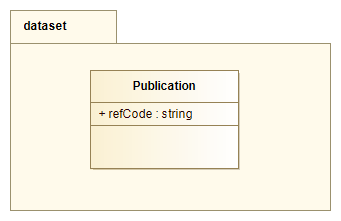
\includegraphics[width=2.375in]{diagrams/Publication.png}
    \caption{ Publication detail diagram}\label{fig:publication}
  \end{center}
  \end{figure}

  Any referenceable publication associated with a Dataset.

  \subsubsection{Publication.refCode}
  \textbf{type: \hyperref[sect:ivoa]{string}} \newline
  \textbf{multiplicity: 1} \newline
  
  Reference code of the publication. Values should be expressed as a URI
  formatted in accordance to an accepted schema. For example: a 'doi' should use
  the form described by the doi schema (http://doi.org); bibcode according to
  the bibcode pattern, namely a 19 character string beginning with 4 digits.
  Free text references are allowed, but discouraged. If used, they must not
  start with the pattern "[a-zA-Z]+:" to ensure they are not interpreted as URIs.
  

\pagebreak
\subsection{Publisher}
\label{sect:publisher}
% ==================

  % INSERT FIGURE HERE
  \begin{figure}[h]
  \begin{center}
    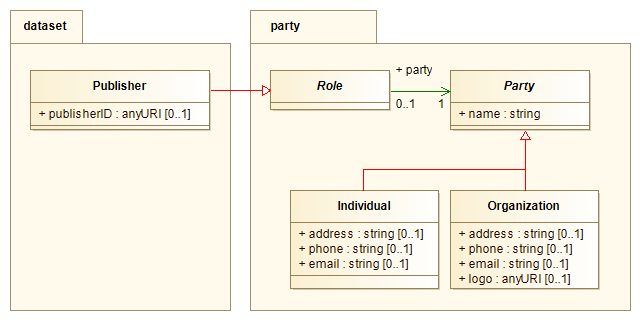
\includegraphics[width=4.75in]{diagrams/Publisher.png}
    \caption{ Publisher detail diagram}\label{fig:publisher}
  \end{center}
  \end{figure}

  Publisher is modeled as a Role played by the organization or entity making the
  Dataset available.

  Party package is described in Section \ref{sect:party_pkg}.

  \subsubsection{Publisher.publisherID}
  \textbf{type: \hyperref[sect:ivoa]{anyURI}} \newline
  \textbf{multiplicity: 0..1} \newline
  
  IVOA resource identifier associated with the publisher and registered with an
  IVOA compliant registry (eg: ivo://mast.stsci.edu). Values are to be expressed
  using the syntax described in "IVOA Identifiers" \citep{2007ivoa.spec.0314P}.
  
% --------------------------------------------------------------------------------
%                                Observation Model
% --------------------------------------------------------------------------------
\pagebreak
\section{Observation-Experiment}
\label{sect:obs}

% INSERT FIGURE HERE
\begin{figure}[h]
\begin{center}
  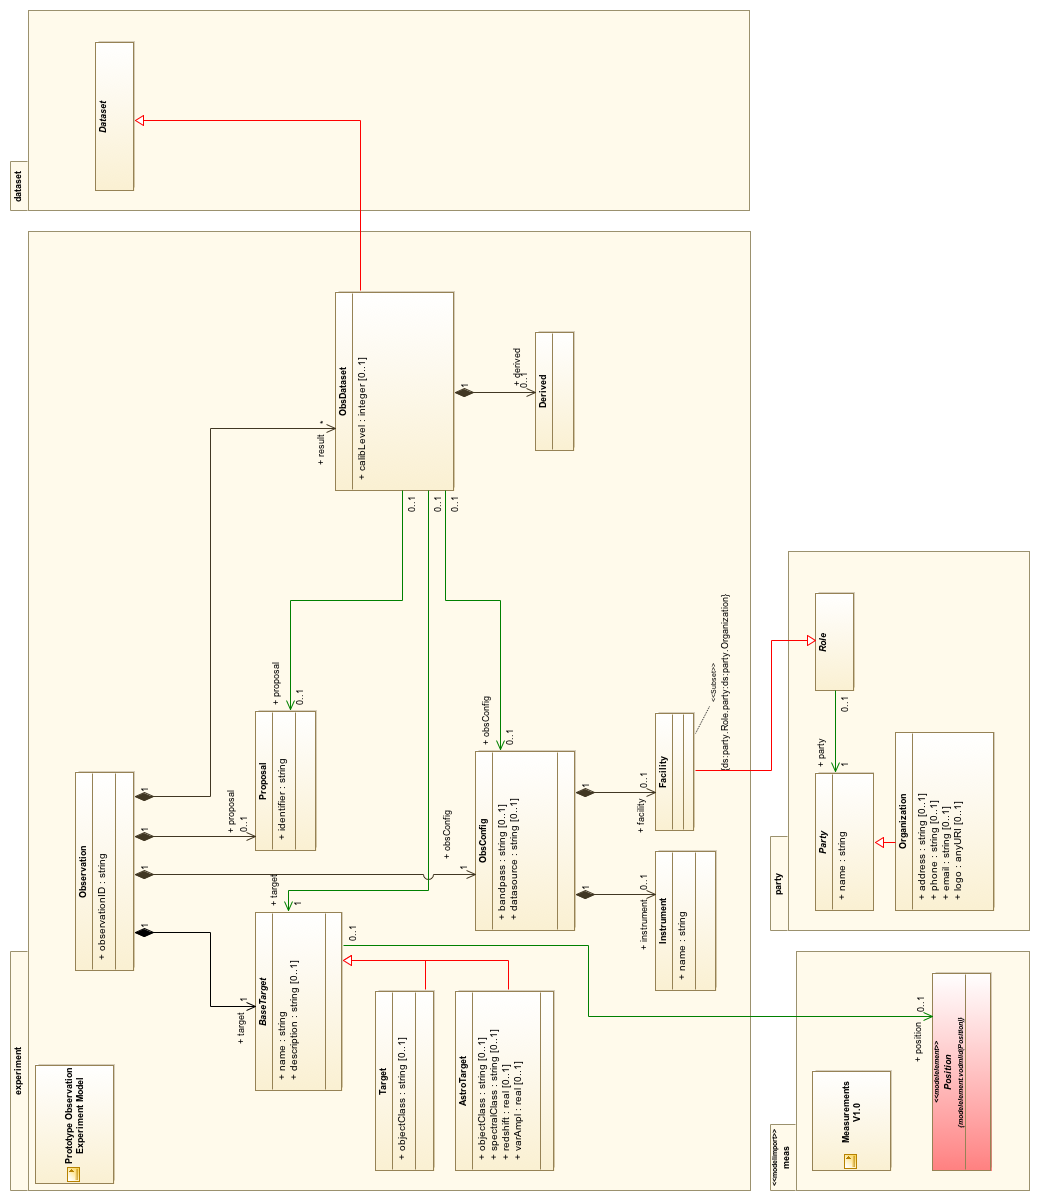
\includegraphics[width=5.5in]{diagrams/Observation_overview.png}
  \caption{Observation/ObsDataset diagram}\label{fig:obs_overview}
\end{center}
\end{figure}

An Observation Dataset (ObsDataset) is modeled as the result of an Observation,
and refers to several elements related to the Observation and its configuration.
As of the time of this writing, there is no IVOA recommendation for a general
Observation data model. The Provenance data model, in progress, will define
the pattern for describing the relation between actions and results, and how
to record these in datasets. In lieu of these standards, this document defines
a strawman Observation model.

\pagebreak
\subsection{Observation}
\label{sect:observation}

  Head class for an Observation Experiment.
  
  The Observation is modeled as a type of 'Experiment', with some basic
  structure defined to provide metadata about the observation target and
  configuration. The product, or 'result' of the Observation is zero or more
  ObsDataset objects. This pattern is inspired by, and compatible with the
  Simulation Data Model \citep{2012ivoa.spec.0503L}, where a 'Simulation' can be considered another form
  of 'Experiment' or perhaps even another form of 'Observation'.

  \subsubsection{Observation.observationID}
  \textbf{type: \hyperref[sect:ivoa]{string}} \newline
  \textbf{multiplicity: 1} \newline

  Internal ID determined by the data provider to uniquely identify the
  observation within the institution or entity performing the observation.  
  
  \subsubsection{Observation.target}
  \textbf{type: \hyperref[sect:basetarget]{BaseTarget}} \newline
  \textbf{multiplicity: 1} \newline

  The target of the observation. The content of this object may vary greatly
  depending on the goals and nature of the observation. For example, the
  'target' could be a galaxy, stellar object, planet, or calibration source. As
  such, we allow the BaseTarget class here, and permit users to define and use
  more content rich flavors according to their needs.
  
  \subsubsection{Observation.obsConfig}
  \textbf{type: \hyperref[sect:obsconfig]{ObsConfig}} \newline
  \textbf{multiplicity: 1} \newline

  Observation configuration metadata, provides information about who, where,
  and how the observation was conducted.
  
  \subsubsection{Observation.proposal}
  \textbf{type: \hyperref[sect:proposal]{Proposal}} \newline
  \textbf{multiplicity: 0..1} \newline

  Identifies any proposal related to the observation. This field may be used
  to gather all observations and products related to a particular proposal.
  
  \subsubsection{Observation.result}
  \textbf{type: \hyperref[sect:obs_ds]{ObsDataset}} \newline
  \textbf{multiplicity: 0..*} \newline

  The result of an observation is zero or more Observation Datasets.
  
  
\subsection{ObsDataset}
\label{sect:obs_ds}

  ObsDataset is an extension of Dataset defining additional metadata relevant to
  Datasets which are derived from Observations. This metadata gives a high-level
  summary of the coverage of the dataset in coordinate space, as well as the
  coordinate systems used, and general information about the observation itself.

  \subsubsection{ObsDataset.calibLevel}
  \textbf{type: \hyperref[sect:ivoa]{integer}} \newline
  \textbf{multiplicity: 0..1} \newline

  High level classification for the calibration level of a particular dataset
  as a whole. The calibration level concept conveys to the user information on
  how much data reduction/processing has been applied to the data. It is up to
  the data providers to consider how to map their own internal classification to
  the scale defined here.
  
  Scale:
  \begin{itemize}
  \item[] 0 - Raw instrumental data, in a proprietary or internal data-provider defined format.
  \item[] 1 - Instrumental data in a standard format (FITS, VOTable, etc )
  \item[] 2 - Calibrated, science ready data with the instrument signature removed.
  \item[] 3 - Enhanced data products like mosaics, resampled or drizzled images,
              or heavily processed survey fields. Level 3 data products may represent the
              combination of data from multiple primary observations.
  \end{itemize}
  
  \subsubsection{ObsDataset.derived}
  \textbf{type: \hyperref[sect:derived]{Derived}} \newline
  \textbf{multiplicity: 0..1} \newline

  Provides a high level summary of certain properties of the dataset. Its
  primary purpose is to support high level filtering of datasets during data
  discovery.
  
  \subsubsection{ObsDataset.obsConfig}
  \textbf{type: \hyperref[sect:obsconfig]{ObsConfig}} \newline
  \textbf{multiplicity: 0..1} \newline

  Reference to ObsConfig object from Observation. This object provides some
  high-level metadata related to the observation configuration.
  
  \subsubsection{ObsDataset.observationID}
  \textbf{type: id} \newline
  \textbf{multiplicity: n/a} \newline

  Implicit element of the ObsDataset object due to the composition relation to
  Observation. This is an internal ID determined by the data provider to
  identify the Observation from which the dataset was produced.
  
  \subsubsection{ObsDataset.proposal}
  \textbf{type: \hyperref[sect:proposal]{Proposal}} \newline
  \textbf{multiplicity: 0..1} \newline

  Reference to Proposal object from Observation. This object provides metadata
  identifying any proposal related to the observation which produced the dataset.  
  
  \subsubsection{ObsDataset.target}
  \textbf{type: \hyperref[sect:basetarget]{BaseTarget}} \newline
  \textbf{multiplicity: 1} \newline
  
  Reference to a BaseTarget object from Observation. Provides metadata
  describing the target of the observation.
  
\pagebreak
% INSERT FIGURE HERE
\begin{figure}[h]
\begin{center}
  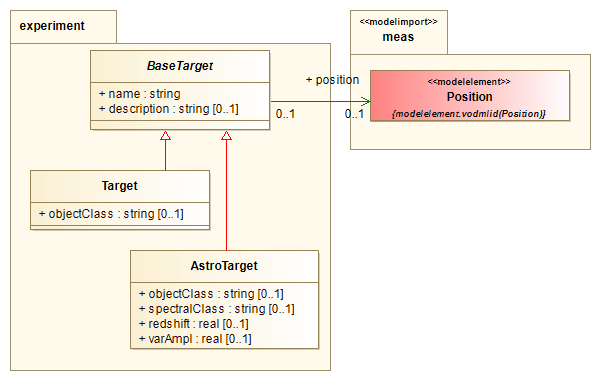
\includegraphics[width=5.0in]{diagrams/Target.png}
  \caption{ Target hierarchy detail diagram}\label{fig:target}
\end{center}
\end{figure}
  
\subsection{AstroTarget}
\label{sect:astrotarget}

  Extension of BaseTarget specialized for astronomical objects. The AstroTarget
  defines additional astronomical properties of the target.

  \subsubsection{AstroTarget.name}
  \textbf{type: \hyperref[sect:ivoa]{string}} \newline
  \textbf{multiplicity: 1} \newline

  When referring to an astronomical target, one may specify a particular
  object, or a more general target such as the name of a survey field. When
  specifying a particular object, it is highly recommended to use a name
  suitable for input to a name resolver.
  
  \subsubsection{AstroTarget.position}
  \textbf{type: \hyperref[sect:pos]{Position}} \newline
  \textbf{multiplicity: 0..1} \newline

  In the context of the astronomical target, this field gives the nominal RA and
  Dec location for the target. For example, the catalog position of the
  source.  
  
  \subsubsection{AstroTarget.objectClass}
  \textbf{type: \hyperref[sect:ivoa]{string}} \newline
  \textbf{multiplicity: 0..1} \newline

  General classification or type of the target. This field supports the
  discovery of data pertaining to a common class of object, e.g. "Star", "
  Galaxy", "AGN". At the time of this writing, there is no IVOA recommended
  vocabulary for this field. The SIMBAD and NED databases use defined
  vocabularies for astronomical object classifications which may serve as the
  basis for such.
  
  \subsubsection{AstroTarget.spectralClass}
  \textbf{type: \hyperref[sect:ivoa]{string}} \newline
  \textbf{multiplicity: 0..1} \newline

  Spectral class of the object. As with objectClass, there is no IVOA
  recommended vocabulary for specifying the spectral class of an object. There
  is an IVOA Note on the subject entitled "An encoding system to represent
  stellar spectral classes in archival databases and catalogs" \citep{note:SpectralClasses},
  describing an encoding system which has been adopted by the MAST archive.  
  
  \subsubsection{AstroTarget.redshift}
  \textbf{type: \hyperref[sect:ivoa]{real}} \newline
  \textbf{multiplicity: 0..1} \newline

  This field gives the canonical redshift of the astronomical object. It is
  normally used to store the cosmological redshift of extragalactic objects,
  although it may also be used to store the observed redshift of Galactic
  sources if that information is felt by the data provider to be useful.  
  
  \subsubsection{AstroTarget.varAmpl}
  \textbf{type: \hyperref[sect:ivoa]{real}} \newline
  \textbf{multiplicity: 0..1} \newline

  Canonical variability amplitude attributed to the target.


\pagebreak
\subsection{BaseTarget}
\label{sect:basetarget}

  Abstract base class for the Target object tree. The target object provides
  identifying metadata related to the subject or goal of the experiment. For an
  Observational experiment, this would typically be an astronomical object. The
  BaseTarget class defines high-level identifying information, and must be
  extended for particular classes of Target which may define additional characteristics.

  \subsubsection{BaseTarget.name}
  \textbf{type: \hyperref[sect:ivoa]{string}} \newline
  \textbf{multiplicity: 1} \newline

  The target name. The primary purpose of this field is to provide the user with
  a recognizable identity of the particular subject or goal. However, since this
  may be a query-able field in data discovery protocols, care should be taken to
  use values which follow conventions for the domain appropriate for the data.
  For an astronomical object, this may be a name suitable for use within a
  domain-specific resolution service. Simulated data might also use this sort of
  name (if simulating a particular object), or a more generic term such as "G2V star".
  
  \subsubsection{BaseTarget.description}
  \textbf{type: \hyperref[sect:ivoa]{string}} \newline
  \textbf{multiplicity: 0..1} \newline

  Free form description of target.
  
  \subsubsection{BaseTarget.position}
  \textbf{type: \hyperref[sect:pos]{Position}} \newline
  \textbf{multiplicity: 0..1} \newline

  This field provides the spatial location of the target. The value is a
  Position object which supports all required dimensionality and coordinate
  frame specification needs.
  
\pagebreak
\subsection{Derived}
\label{sect:derived}

  % INSERT FIGURE HERE
  \begin{figure}[h]
  \begin{center}
    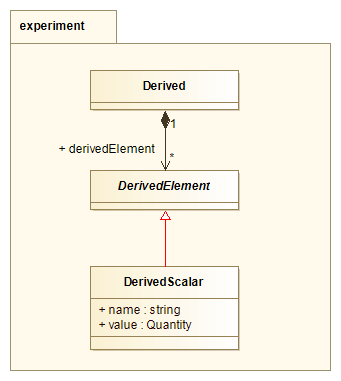
\includegraphics[width=2.625in]{diagrams/Derived.png}
    \caption{ Derived detail diagram}\label{fig:derived}
  \end{center}
  \end{figure}

  The Derived (short for Derived Data) object holds derived information obtained
  by evaluating or analyzing the contents of the dataset. The specific content
  of this object is strongly dependent on the specific type of dataset, so we
  provide a generic model which may be specialized in other models to define
  elements appropriate for that type of dataset.
  
  The primary purpose of this object is to provide a common framework in which
  specific information may be placed to aid in discovery and filtering of
  datasets in various access protocols.

  \subsubsection{DerivedScalar.derivedElement}
  \textbf{type: \hyperref[sect:derived_element]{DerivedElement}} \newline
  \textbf{multiplicity: 0..*} \newline

  Collection of zero or more DerivedElement objects, each of which provides a
  specific quantity obtained by analyzing the dataset content.
  
\subsection{DerivedElement}
\label{sect:derived_element}

Abstract base for defining derived data elements. Typically, models for
specific data products would extend this object to define various elements
appropriate for that model. For example, the Spectrum model could define
signal-to-noise ratio (SNR), or TimeSeries could define period, or
variability. We put no restriction on the DerivedElement content since the
result could be a simple value or a complex object. However, it is recommended
that extensions be simple and compact in keeping with the primary intent of
use in data discovery.

\subsection{DerivedScalar}
\label{sect:derived_scalar}
Simple extension of DerivedElement class which can serve many use cases.
Usages of this object in other models to define specific elements should
explicitly define the element name, and the process by which the value is
determined.

  \subsubsection{DerivedScalar.name}
  \textbf{type: \hyperref[sect:ivoa]{string}} \newline
  \textbf{multiplicity: 1} \newline

  Name identifying the derived element.
  
  \subsubsection{DerivedScalar.value}
  \textbf{type: \hyperref[sect:ivoa]{Quantity}} \newline
  \textbf{multiplicity: 1} \newline

  Value of the derived element.

\pagebreak
% INSERT FIGURE HERE
\begin{figure}[h]
\begin{center}
  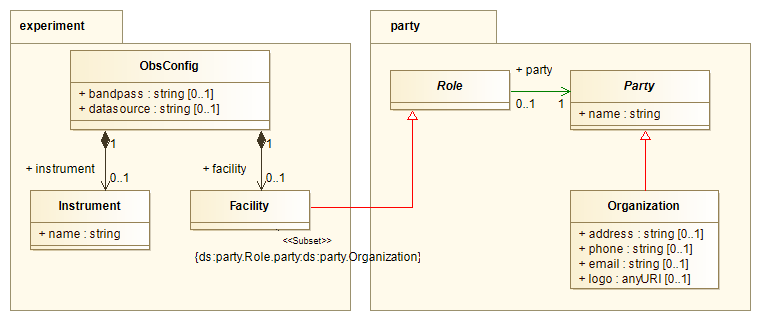
\includegraphics[width=5.125in]{diagrams/ObsConfig.png}
  \caption{ ObseConfig detail diagram}\label{fig:obsconfig}
\end{center}
\end{figure}
  
\subsection{Facility}
\label{sect:facility}

The Facility performing the observation. This is modeled as the Role played by
a particular Organization (Party entity).

\subsection{Instrument}
\label{sect:instrument}

The instrument used to create the data. This can be a specific instrument,
general type or something else, such as a program in the case of theoretical
data. (RM:Collection.Instrument)

\subsection{ObsConfig}
\label{sect:obsconfig}

ObsConfig describes all Observation Configuration metadata. We define a small
set of configuration elements which are required as Provenance in the
observation dataset.

  \subsubsection{ObsConfig.bandpass}
  \textbf{type: \hyperref[sect:ivoa]{string}} \newline
  \textbf{multiplicity: 0..1} \newline

  Describes the Spectral domain of the Observation in very general sense.

  The value may be expressed in terms of general spectral bands, or specific
  bandpass names. If multiple bands are covered, the value may be a comma
  delimited combination of appropriate bands. If expressed as general bands, the
  value(s) must be selected from the enumerated set given by the SpectralBand
  type (Section \ref{sect:band}) . There is no controlled vocabulary for specific
  bandpass names as the list is too long to enumerate. Effort should be made
  to use highly recognized bandpass names (eg: "U","V","B","R","I", "H-alpha").
  
  This field corresponds to both the Coverage.Spectral and Coverage.Spectral.
  Bandpass fields of the Resource Metadata document.
  
  \subsubsection{ObsConfig.dataSource}
  \textbf{type: \hyperref[sect:ivoa]{string}} \newline
  \textbf{multiplicity: 0..1} \newline

  Describes the original source of the data in a very general fashion. In
  other words, ``What sort of observation originally generated the data?''
  Suggested values include:
  \begin{itemize}
  \item \textbf{survey}: Survey data typically covers some region of observational parameter space with as complete as possible coverage within that region.
  \item \textbf{pointed}: Pointed data of a particular object or field.
  \item \textbf{theory}: Theory data, generated based on a theoretical model.
  \item \textbf{artificial}: Artificial, or simulated data. Similar to 'theory', but not necessarily based on a theoretical model.
  \item \textbf{custom}: Custom data, as part of a specific research project.
  \end{itemize}

  \subsubsection{ObsConfig.facility}
  \textbf{type: \hyperref[sect:facility]{Facility}} \newline
  \textbf{multiplicity: 0..1} \newline

  Metadata pertaining to the facility performing the observation.
  
  \subsubsection{ObsConfig.instrument}
  \textbf{type: \hyperref[sect:instrument]{Instrument}} \newline
  \textbf{multiplicity: 0..1} \newline

  Metadata pertaining to the instrument used to create the data.

\pagebreak
\subsection{Proposal}
\label{sect:proposal}

  % INSERT FIGURE HERE
  \begin{figure}[h]
  \begin{center}
    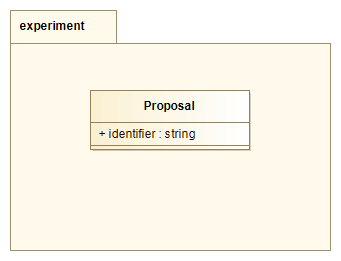
\includegraphics[width=2.375in]{diagrams/Proposal.png}
    \caption{ Proposal detail diagram}\label{fig:proposal}
  \end{center}
  \end{figure}
  
  Metadata related to the proposal or document which spawned the observation.

  \subsubsection{Proposal.identifier}
  \textbf{type: \hyperref[sect:ivoa]{string}} \newline
  \textbf{multiplicity: 0..1} \newline

  Tag used to uniquely identify a particular proposal within the institution or entity.
  
\pagebreak
\subsection{Target}
\label{sect:target}

Extension of BaseTarget, this is a general purpose Target object.

  \subsubsection{Target.objectClass}
  \textbf{type: \hyperref[sect:ivoa]{string}} \newline
  \textbf{multiplicity: 0..1} \newline

  General classification or type of the target. This field supports the
  discovery of data pertaining to a common class of object, e.g. "Star", "
  Galaxy", "AGN". At the time of this writing, there is no IVOA recommended
  vocabulary for this field. The SIMBAD and NED databases use defined
  vocabularies for astronomical object classifications which may serve as the
  basis for such.

% --------------------------------------------------------------------------------
%                                   Party Model
% --------------------------------------------------------------------------------
\pagebreak
\section{Party Package}
\label{sect:party_pkg}

% INSERT FIGURE HERE
\begin{figure}[h]
\begin{center}
  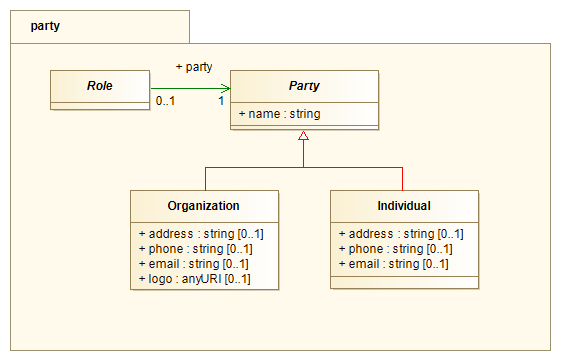
\includegraphics[width=4.125in]{diagrams/Party.png}
  \caption{Party package diagram}\label{fig:party}
\end{center}
\end{figure}

We include a simple Party model for associating an Entity with a Role that
Entity is playing. For example, a particular Individual can be both a
Contact and Publisher of a dataset.

\subsection{Role}
Abstract class for the entity role. Models should extend this class to define
local roles which are played by various entities/parties.

  \subsubsection{Role.party}
  \textbf{type: \hyperref[sect:party]{Party}} \newline
  \textbf{multiplicity: 1} \newline
  
   Reference to the Party or Entity which is associated with this role.

\subsection{Party}
\label{sect:party}
Abstract head of the set of classes describing various entities.

  \subsubsection{Party.name}
  \textbf{type: \hyperref[sect:ivoa]{string}} \newline
  \textbf{multiplicity: 1} \newline
  
  Name of the Party or entity. All entities are assumed to have a name.
  
\subsection{Individual}
Party which describes an individual or representative.

  \subsubsection{Individual.address}
  \textbf{type: \hyperref[sect:ivoa]{string}} \newline
  \textbf{multiplicity: 0..1} \newline
  
  Mailing address for the Individual. The value is expressed as a single string
  containing all components of the address.
  
  \subsubsection{Individual.email}
  \textbf{type: \hyperref[sect:ivoa]{string}} \newline
  \textbf{multiplicity: 0..1} \newline
  
  E-mail address of the Individual.
  
  \subsubsection{Individual.phone}
  \textbf{type: \hyperref[sect:ivoa]{string}} \newline
  \textbf{multiplicity: 0..1} \newline
  
  Phone number associated with the Individual. The value is expressed as a string
  according to the format appropriate for the locale.
  

  \subsection{Organization}
  Extension of Party for any Organization or Institution.
  
  \subsubsection{Organization.address}
  \textbf{type: \hyperref[sect:ivoa]{string}} \newline
  \textbf{multiplicity: 0..1} \newline
  
  Mailing address. The value is expressed as a single string containing all
  components of the address.
    
  \subsubsection{Organization.email}
  \textbf{type: \hyperref[sect:ivoa]{string}} \newline
  \textbf{multiplicity: 0..1} \newline
  
  E-mail address of the Organization.
  
  \subsubsection{Organization.logo}
  \textbf{type: \hyperref[sect:ivoa]{anyURI}} \newline
  \textbf{multiplicity: 0..1} \newline
  
  URL pointer to a graphical logo associated with the Organization.
    
  \subsubsection{Organization.phone}
  \textbf{type: \hyperref[sect:ivoa]{string}} \newline
  \textbf{multiplicity: 0..1} \newline
  
  Phone number. The value is expressed as a string according to the format
  appropriate for the locale.

  

% --------------------------------------------------------------------------------
%                                    Data Types
% --------------------------------------------------------------------------------
\pagebreak
\section{Data Types}
\label{sect:types}

\subsection{Base Data Types}
\label{sect:ivoa}
Provides a set of standardized primitive data types as well as types for
representing quantities ( values with associated units ). We provide a diagram
of the model here, and refer the reader to Section 5 of the VO-DML modeling
specification document\citep{2018ivoa.spec.0910L} for more information.

  % INSERT FIGURE HERE
  \begin{figure}[h]
  \begin{center}
    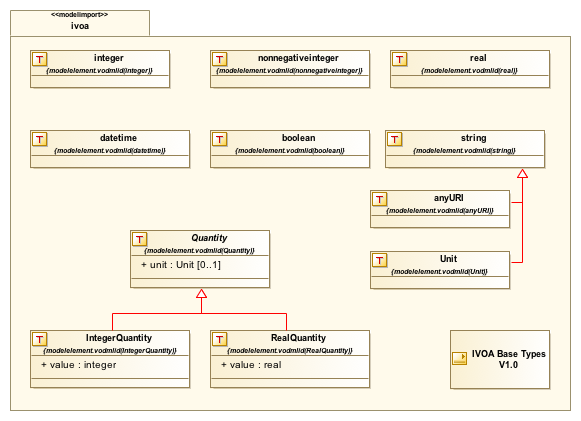
\includegraphics[width=4.875in]{diagrams/BaseTypes.png}
    \caption{Base Data Types}\label{fig:basetypes}
  \end{center}
  \end{figure}

  \subsubsection{Units}
  \label{sect:units}
  This model requires the use of the IVOA VOUnits Standard\citep{2014ivoa.spec.0523D} for representing
  units of physical quantities. This standard reconciles common practices and
  current standards for use within the IVOA community.
  
  \subsubsection{UCDs}
  \label{sect:ucds}
  This model requires any ucd field to comply with syntax defined in ”An IVOA
  Standard for Unified Content Descriptors”\citep{2005ivoa.spec.0819D}.
  
  \subsubsection{Dates}
  \label{sect:dates}
  The 'datetime' datatype is for expressing date-time values. The string
  representation of a datetime value should follow the FITS convention for
  representing dates. The FITS standard is effectively ISO8601 format without
  the "Z" tag to indicate UTC (YYYY-MM-DDThh:mm:ss).
  Values are nominally expressed in UTC.


\pagebreak
\subsection{Dataset Model Data Types}
% ==================================
The Dataset model has gathered and homogenized data type definitions from
previous specifications like ObsCore (DataProductType), VOResource (RightsType),
and VODataservice (SpectralBandType).

  % INSERT FIGURE HERE
  \begin{figure}[h]
  \begin{center}
    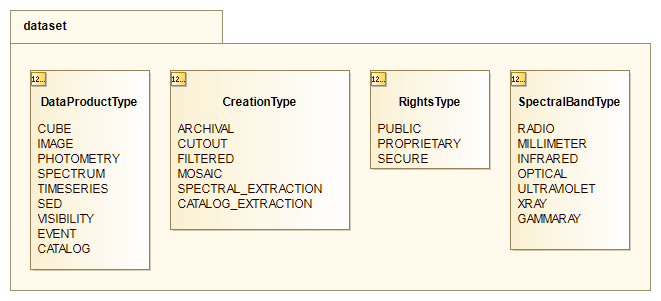
\includegraphics[width=4.0in]{diagrams/DataTypes.png}
    \caption{Dataset model datatypes}\label{fig:dtypes}
  \end{center}
  \end{figure}

  \subsubsection{CreationType}
  \label{sect:creation}
  Enumeration of dataset creation types. Allowed values are:

  \begin{table}[h!]
    \small
    \centering
    \renewcommand{\arraystretch}{1.5}
    \begin{tabular}{|p{1.0in}|p{0.75in}|p{3.5in}|}
      \hline 
           \textbf{Token} & \textbf{Label} & \textbf{Meaning}\\
      \hline  
      \hline  
      ARCHIVAL  & archival & Indicates that it is one of a collection of datasets generated in a systematic, homogeneous way and is stored statically (or at least versioned). It will be possible to regenerate this dataset at a later date. The remaining types imply on-the-fly manipulation. \\
      \hline  
      CUTOUT    & cutout   & Indicates that the dataset was created "on-the-fly", by subsetting, but not by modifying values. \\
      \hline  
      FILTERED  & filtered & May involve excluding data prior to binning into samples, also "on-the-fly" \\
      \hline  
      MOSAIC    & mosaic   & Combines multiple original datasets "on-the-fly" \\
      \hline  
      SPECTRAL\_ EXTRACTION & spectral extraction & Has been extracted, for example, from a spectral data cube. \\
      \hline  
      CATALOG\_ EXTRACTION  & catalog extraction  & Has been extracted from a catalog. \\
      \hline 
    \end{tabular}
  \end{table}

  
  \pagebreak
  \subsubsection{DataProductType}
  \label{sect:product}
  Enumeration identifying the high level classification of a data product. Allowed values are:

  \begin{table}[h!]
    \small
    \centering
    \renewcommand{\arraystretch}{1.5}
    \begin{tabular}{|p{1.25in}|p{0.75in}|p{3.5in}|}
      \hline 
           \textbf{Token} & \textbf{Label} & \textbf{Meaning}\\
      \hline  
      \hline  
      CUBE       & cube       &  A multidimensional astronomical image of three (3) or more axes. \\
      \hline  
      IMAGE      & image      &  A two (2) dimensional astronomical image. \\
      \hline  
      PHOTOMETRY & photometry &  Dataset with spectral coverage with irregular gaps. \\
      \hline  
      SPECTRUM   & spectrum   &  Dataset where spectral coverage is the primary attribute, in contiguous bins. e.g. a 1D spectrum or a long slit spectrum. \\
      \hline  
      TIMESERIES & timeseries &  Dataset presenting some quantity varying as a function of time. A light curve is a typical example of a timeseries dataset. \\
      \hline  
      SED        & sed        &  A spectral energy distribution, an advanced data product often produced by combining data from multiple observations. \\
      \hline  
      VISIBILITY & visibility &  A visibility (radio) dataset. Typically this is instrumental data, and is often a complex object containing multiple files or other substructures. A visibility dataset may contain data with spatial, spectral, time, and polarization information for each measured visibility. \\
      \hline  
      EVENT      & event      &  An event counting dataset (e.g. X-ray). An event dataset may contain data with spatial, spectral, and time information for each measured event. \\
      \hline  
      CATALOG    & catalog    &  A catalog. \\
      \hline 
    \end{tabular}
  \end{table}

  \subsubsection{RightsType}
  \label{sect:rights}
  Enumeration indicating access rights levels. Allowed values are:

  \begin{table}[h!]
    \small
    \centering
    \renewcommand{\arraystretch}{1.5}
    \begin{tabular}{|p{1.25in}|p{0.75in}|p{3.5in}|}
      \hline 
           \textbf{Token} & \textbf{Label} & \textbf{Meaning}\\
      \hline  
      \hline  
      PUBLIC      & public      & unrestricted, public access is allowed, without authentication. \\
      \hline  
      SECURE      & secure      & authenticated, public access is allowed. \\
      \hline  
      PROPRIETARY & proprietary & only proprietary access is allowed with authentication. \\
      \hline  
    \end{tabular}
  \end{table}
  
  \subsubsection{SpectralBandType}
  \label{sect:band}
  Enumeration of generic spectral bands:
  
  \begin{table}[h!]
    \small
    \centering
    \renewcommand{\arraystretch}{1.5}
    \begin{tabular}{|p{1.25in}|p{0.75in}|p{3.5in}|}
      \hline 
           \textbf{Token} & \textbf{Label} & \textbf{Meaning} ( $\lambda$=wavelength, $\nu$=frequency, E=energy) \\
      \hline  
      \hline  
      RADIO       & Radio       & $\lambda \geq$ 10 mm; $\nu \leq$ 30 GHz \\
      \hline  
      MILLIMETER  & Millimeter  & 0.1 mm $\leq \lambda \leq$ 10 mm; 3000 GHz $\geq \nu \geq$ 30 GHz \\
      \hline  
      INFRARED    & Infrared    & 1 $\mu \leq \lambda \leq$ 100 $\mu$ \\
      \hline  
      OPTICAL     & Optical     & 0.3 $\mu \leq \lambda \leq$ 1 $\mu$ \\
      \hline  
      ULTRAVIOLET & Ultraviolet & 100 \AA $\leq \lambda \leq$ 3000 \AA; 1.2 eV $\leq$ E $\leq$ 120 eV \\
      \hline  
      XRAY        & X-ray       & 0.1 \AA $\leq \lambda \leq$ 100 \AA; 0.12 keV $\leq$ E $\leq$ 120 keV \\
      \hline  
      GAMMARAY    & Gamma-ray   & E $\geq$ 120keV \\
      \hline  
    \end{tabular}
  \end{table}
  

% --------------------------------------------------------------------------------
%                              External Dependencies
% --------------------------------------------------------------------------------
\pagebreak
\section{Measurements Data Model}
\label{sect:meas}

This model uses (imports) elements from the Measurements data model. This
section gives a brief description of the elements used. This content is for
reference only, the model document is considered normative and supercedes any
descriptions provided here.

\pagebreak
\subsection{Physical Measurements (Meas)}

  % INSERT FIGURE HERE
  \begin{figure}[h]
  \begin{center}
    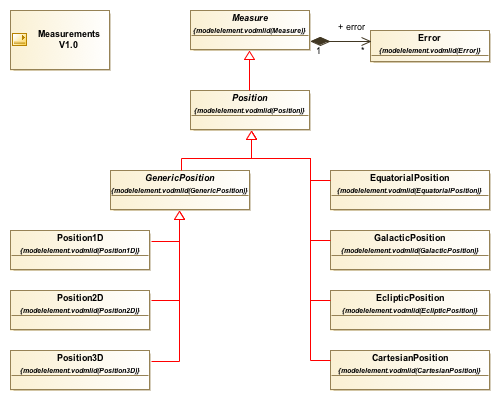
\includegraphics[width=4.5in]{diagrams/Measurement_elements.png}
    \caption{Measurement model elements}\label{fig:measurements}
  \end{center}
  \end{figure}

  \subsubsection{Position}
  \label{sect:pos}
  Provides a physical location in a spatial coordinate space. The measurements
  model provides a generic position type as well as several specialized types
  for the most common cases. This model is not limited to the set shown here,
  and may take any Position type.

  



\pagebreak
\section{Changes from Previous Versions}
% No previous versions yet.  

% these would be subsections "Changes from v. WD-..."
% Use itemize environments.
% ------------------------------------
%\subsection{Changes from WD-YYYY-MM-DD}
%\begin{itemize}
%\item Add Change List
%\end{itemize}
% ------------------------------------

\subsection{Changes from initial draft WD-2014-06-13}
\begin{itemize} % 2014 Sep 30:
  \item  Draft revised with STC2 prototype, initial draft feedback, and updates due to Cube model development.
\end{itemize}

\subsection{Changes from WD-2014-09-30}
\begin{itemize} % 2015 Mar 02
  \item Incorporate comments from Spectral2.0 feedback related to Dataset metadata.
  \item Format change to better illustrate data type and multiplicity of elements.
  \item Update STC2 prototype to current state of development.
  \item General review of element descriptions for clarity.
\end{itemize}

\subsection{Changes from WD-2015-03-02}
\begin{itemize} % 2015 Oct 07
  \item Update Acknowledgments for European contributors
  \item Generalize Derived object using ObsConfig pattern
  \item Remove Redshift type (used in Derived)
  \item Update STC2 prototype to 2015-05-04 model descriptions (except for Transform model)
  \item Update reference to VO-DML specification (2015-02-06 version) - Make section references links.
\end{itemize}

\subsection{Changes from WD-2015-10-07}
\begin{itemize} % 2015 Oct 18
  \item Update STC2 prototype to 2015-10-14 model diagrams
  \begin{itemize}
    \item Frame - Transform relation. 2016 Mar 09:
  \end{itemize}
  \item Update elements for vo-dml compatibility
  \begin{itemize}
    \item Curation.reference, DataID.collection, DataID.contributor o Enumerations (SpectralBandType)
  \end{itemize}
  \item Added simple Party model for Entity types
  \begin{itemize}
    \item Curation.publisher, Curation.contact, DataID.creator, DataID.contributor
  \end{itemize}
  \item Restructured ObsConfig, folding in content concepts, not just content. - Normalized Curation.rights from string to AccessRights type.
  \item Update STC2 prototype
  \begin{itemize}
    \item duplicate packaging
    \item mods for vo-dml compliance, PixelSpace, PixelCoordinate, Transforms. 2016 Apr 12:
  \end{itemize}
  \item restore Curation.rights to attribute of type RightsType, delete AccessRights type.
  \item reduce Party types to just Organization and Individual.
  \item enhanced language in Publication.refCode description.
  \item moved ObsDataset and associated elements to Observation-Experiment package - added list of figures
\end{itemize}

\subsection{Changes from WD-2015-10-18}
\begin{itemize} % 2016 Oct 31
  \item remove STC2 prototype model
\end{itemize}

%\subsection{Changes from WD-2016-10-31}
\begin{itemize} % 2017 Sep 27
  \item removed Characterisation element from ObsDataset; belongs on specific dataset types.
  \item removed CoordSys element from ObsDataset; convenience element for content defined elsewhere.
  \item update to current STC2 Measurement model interface
\end{itemize}

\subsection{Changes from WD-2017-09-27}
\begin{itemize} % 2019 Sep 17
  \item update to Measurements model (minor); and stereotype URLs.
\end{itemize}

\subsection{Changes from WD-2019-09-17}
\begin{itemize} % 2022 Dec 13
  \item migration to ivoatex
\end{itemize}



\appendix
% Appendix A: for UML diagram conventions
\pagebreak
\section{Modeling Conventions}

\subsection{Diagram Notation}
This model follows the VO-DML modeling practices, however, the UML
representations may vary depending on the tool used.  Below we describe the
graphical representation of the modeling concepts and relations.


  \begin{figure}[h]
  \begin{center}
    \fbox{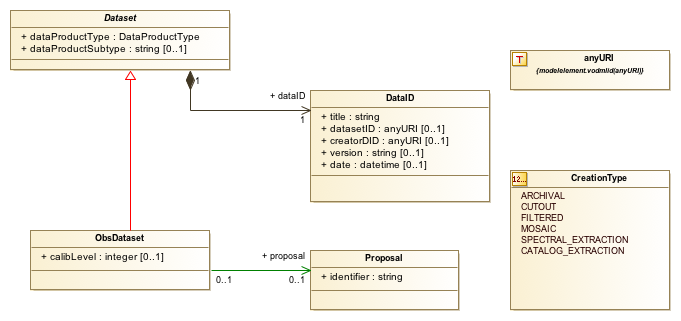
\includegraphics[width=0.9\textwidth]{diagrams/notation_example.png}}
    \caption{Notation example diagram}\label{fig:notation_example}
  \end{center}
  \end{figure}

  \subsubsection{ObjectType}
  \label{sect:ObjectType}
  ObjectTypes are represented by a plain box. The type name is annotated in the top window, abstract
types use italic typeface. Attributes, if any, are listed in the lower panel. Attributes may only be
of primitive type (real, string, etc), a defined DataType, or an Enumeration type. Relationships to
other objects are defined via the composition and reference relation arrows.

  \subsubsection{DataType}
  \label{sect:DataType}
  DataTypes are represented by a box shape similar to ObjectType, but annotated with a "T" symbol in the top left corner.

  \subsubsection{Enumerations}
  \label{sect:Enumerations}
  Enumerations are represented by a box shape similar to ObjectType, but annotated with a "1,2.."
symbol in the top left corner. Enumeration Literals (possible values) are listed below the
enumeration type name.

  \subsubsection{Generalization}
  \label{sect:Generalization}
  Generalizations are represented by a red line, with open triangle at the end of the source, or more general, object.

  \subsubsection{Composition}
  \label{sect:Composition}
  The composition relation is indicated by a black line with a solid diamond attached to the
containing object, and an arrow pointing to the object being contained. The composition relation is
very tight, where the container is responsible for the creation and existence of the target. Any
object may be in no more than one composition relation with any container. The attribute name
for the composition relation is annotated at the destination of the relation (e.g. "+ dataID"). This is
typically a lower-cased version of the destination type name, but this is not required.

  \subsubsection{Reference}
  \label{sect:Reference}
  The reference relation is indicated by a green line, with an arrow pointing to the object being
referenced. The reference relation is much looser than composition, the container has no
ownership of the target, but merely holds a pointer, or other indirect connection to it. The
attribute name is annotated at the destination of the relation ( e.g. "+ proposal"). This is typically
a lower-cased version of the destination type name, but may be another name indicating the role
that the element is playing in this context.

  \subsubsection{Multiplicity}
  \label{sect:Multiplicity}
  All attributes and relations have a multiplicity associated with them. For attributes, the multiplicity
is contained within brackets just after the attribute name. If no bracket is displayed, this is
equivalent to '[1]'.
\begin{itemize}
\item 1 = one and only one value must be provided.
\item 0..1 = zero or one value may be provided.
\item * = zero or more values may be provided (open ended).
\end{itemize}


\pagebreak
\subsection{Model Identification metadata}
\label{sect:stereotypes}

Interoperability of datasets requires that there be a standardized method for
identifying the specific type of dataset, and which model(s) and versions
thereof it conforms to. These elements are not properties of the dataset, but
rather, of the Model itself. We provide this information via stereotypes
assigned to the model packages (e.g. Dataset, Char, Meas, IVOA ).

  \subsubsection{Model stereotype}
  The Model stereotype (<<model>>) consists of a set of Model properties which
  identify a particular model and its dependencies. Each model should
  specifically state the appropriate values for these properties.

  \begin{itemize}
  \item \textbf{title:string[1]} \newline
    The model title or long name.
  \item \textbf{version:string[1]} \newline
    The version of this model. To be represented as a string with format "<version>.<subversion>"
  \item \textbf{name:string[1]} \newline
    Sometimes referred to as 'namespace’ or 'prefix', this is a tag which is
    used to label elements of a particular model. The value must match the name of
    the model package itself. This string identifies the particular model type 
    (eg. ds, char, meas). Each model must declare a prefix string which is
    unique within the IVOA to tag elements from those models. A typical use of the
    prefix is in the construction of element UTYPE strings.
  \item \textbf{url:anyURI[1]} \newline
    A URL from which the full model description may be obtained (e.g. XML schema).
  \item \textbf{imports:Import[*]} \newline
    Here, we specify which the models on which this model is dependent. This
    model uses and/or extends elements from the Characterisation and Measurements
    Data models. In this document, we provide descriptions and supporting
    information about usage of these objects in a particular context. The
    originating documents, however, remain the definitive source for element definitions.
  \end{itemize}

  \subsubsection{ImportStereotype}
  The <<modelimport>> stereotype is attached to Packages representing imported
  models. It identifies the model by name, and provides URLs from which the full
  description may be obtained.
  \begin{itemize}
  \item \textbf{name:string[1]} \newline
    The name of the imported model. This name MUST match the 'name' property of
    imported model's Model metadata.
  \item \textbf{version:string[1]} \newline
    The version of this model. To be represented as a string with format "<version>.<subversion>"
  \item \textbf{url:anyURI[1]} \newline
    A URL from which the full model description may be obtained (e.g. XML schema).
  \end{itemize}
  

\pagebreak
\subsection{Extensibility}
There is no formal mechanism in the IVOA defining how users may extend models
with their own content. However, the above Model identification metadata
provides a simple means to do so. Using this process, a user would model their
content as an extension of the IVOA standard.

  \subsubsection{Model}
    \begin{itemize}
    \item \textbf{name} \newline
      The user-defined model would need a name unique from that of the standard.
    \item \textbf{prefix} \newline
      A unique prefix must be defined for the user-defined model elements. Users
      must take care not to make use of prefix tags which are associated with
      current IVOA standards, (e.g. ’cha’, ’spec’, ’ssa’, ’meas’). At the time of
      this writing, there is no central repository of reserved namespace strings.
    \item \textbf{imports} \newline
      The user defined model should declare the IVOA standard being extended as
      an imported model. Fields for the imported model name and url may be obtained
      from that standard's documentation.
    \end{itemize}

  \subsubsection{Scope}
  We permit any object modeled in this document to be extended with user-
  defined content, with the following restrictions:
  \begin{itemize}
  \item Follow VO-DML modeling practices.
  \item Values of extended content must be consistent with the content of
        modeled data. That is, using the IVOA base primitive types, Quantity,
        and Coordinates as appropriate.
  \item Since extended content, by definition, does not follow the
        corresponding model, it is not possible for general applications to
        interpret complex structures within that content. It is, therefore,
        recommended that users define extended content in such a way as to
        avoid ambiguity between its components.
  \end{itemize}

  \subsubsection{Support}
  Applications should, but are not required to, provide the following support for extended content:
  \begin{itemize}
  \item Retain existence of extended content, including namespace and UTypes.
  \item Retain association with modeled component.
  \item Provide access to extended content by users.
  \end{itemize}
  


% Appendix B: summary table
\section{Dataset Metadata Model Summary}

\begin{landscape}
{
  \begin{flushleft}
  
  \begin{table}[h!]
    \tiny
    \renewcommand{\arraystretch}{1.5}
    \begin{tabular}{|p{2.5in}|p{1.0in}|p{0.5in}|p{2.25in}|p{2.5in}|}
      \hline
      \multicolumn{5}{|c|}{ \textbf{Dataset Model Identification } } \\
      \hline 
      \textbf{Model Element} & \textbf{Datatype} & \textbf{Mult.} & \textbf{Meaning} & \textbf{Value} \\
      \hline  
        \textbf{Model identification} &         &   &                                                 &   \\
        Model                         &         &   &                                                 &   \\
        model.title                   & string  & 1 & Data model name                                 & "Dataset Metadata"  \\
        model.version                 & string  & 1 & Data model version                              & "1.0"  \\
        model.name                    & string  & 1 & Data model short name, prefix tag               & "ds"  \\
        model.url                     & anyURI  & 1 & Reference URL for model                         & <TBD>  \\
        \textbf{Imported Model}       &         &   &                                                 &   \\
        modelimport.name              & string  & 1 & Imported model name                             & "meas"  \\
        modelimport.version           & string  & 1 & Imported model version                          & "2.0"  \\
        modelimport.url               & anyURI  & 1 & Reference URL for imported model                & https://volute.g-vo.org/svn/trunk/projects/dm/STC/ Meas/vo-dml/STC\_meas-v1.0.vo-dml.xml  \\
        modelimport.documentationURL  & anyURI  & 1 & Reference URL for imported model documentation  & https://volute.g-vo.org/svn/trunk/projects/dm/STC/ Meas/vo-dml/STC\_meas-v1.0.html  \\
        \textbf{Imported Model}       &         &   &                                                 &   \\
        modelimport.name              & string  & 1 & Imported model name                             & "ivoa"  \\
        modelimport.version           & string  & 1 & Imported model version                          & "1.0"  \\
        modelimport.url               & anyURI  & 1 & Reference URL for imported model                & http://www.ivoa.net/xml/VODML/IVOA-v1.vo-dml.xml  \\
        modelimport.documentationURL  & anyURI  & 1 & Reference URL for imported model documentation  & "https://volute.g-vo/svn/trunk/projects/dm/vo-dml/models/ivoa/vo-dml/IVOA-v1.0.html"  \\
      \hline 
    \end{tabular}
  \end{table}

  {
    \tiny
    \renewcommand{\arraystretch}{1.5}
    
    \begin{longtable}[h!]{|p{2.5in}|p{1.0in}|p{0.5in}|p{2.25in}|p{2.5in}|}
      \hline
      \multicolumn{5}{|c|}{ \textbf{Dataset Model Summary } } \\
      \hline 
      \textbf{Model Element} & \textbf{Datatype} & \textbf{Mult.} & \textbf{Meaning} & \textbf{UCD1+} \\
      \hline
      \endfirsthead
    
      \hline
      \multicolumn{5}{|c|}{ \textbf{Dataset Model Summary - Continued } } \\
      \hline 
      \textbf{Model Element} & \textbf{Datatype} & \textbf{Mult.} & \textbf{Meaning} & \textbf{UCD1+} \\
      \hline
      \endhead
    
      \hline
      \endfoot
    
      \hline
      \endlastfoot
    
      % Table content
      \textbf{Dataset Model Elements}     &                     &      &                                                              & \\
      Collection                          & Collection          &      & Descriptive metadata of a compatible grouping                & \\
      Collection.name                     & string              & 1    & Collection name                                              & \\
      Contact                             & Contact             &      & Extension of party Role. Entity to contact for assistance.   & \\
      Contact.party                       & Individual          & 0..1 & Entity associated with Contact role.                         & \\
      Contributor                         & Contributor         &      & Extension of Role. Entity participated in dataset generation & \\
      Contributor.acknowledgement         & string              & 1    & Acknowledgment expression for the contributor                & \\
      Creator                             & Creator             &      & Extension of Role. Entity which created the dataset          & \\
      Curation                            & Curation            &      &                                                              & \\
      Curation.contact                    & Contact             & 0..1 & Contact entity for curation service                          & \\
      Curation.publisher                  & Publisher           & 1    & Publisher                                                    & meta.curation \\
      Curation.publisherDID               & anyURI              & 0..1 & Publisher specified dataset ID                               & meta.ref.url;meta.curation \\
      Curation.reference                  & Publication         & 0..* & Reference to publication associated with the dataset         & \\
      Curation.releaseDate                & datetime            & 0..1 & Date curated dataset last modified                           & time.release \\
      Curation.rights                     & RightsType          & 0..1 & Level of access granted                                      & meta.code \\
      Curation.version                    & string              & 0..1 & Publisher version of the dataset                             & meta.version;meta.curation \\
      DataID                              & DataID              &      &                                                              & \\
      DataID.collection                   & Collection          & 0..* & Collection(s) to which the dataset is a member               & meta.id \\
      DataID.contributor                  & Contributor         & 0..* & Contributor(s)                                               & \\
      DataID.creationType                 & CreationType        & 0..1 & Dataset creation type                                        & \\
      DataID.creator                      & Creator             & 0..1 & Institution or entity which created the dataset              & meta.curation \\
      DataID.creatorDID                   & anyURI              & 0..1 & Creator defined Dataset Identifier                           & meta.id \\
      DataID.datasetID                    & anyURI              & 0..1 & IVOA Dataset Identifier                                      & meta.id;meta.dataset \\
      DataID.date                         & datetime            & 0..1 & Data processing/creation date                                & time.epoch;meta.dataset \\
      DataID.title                        & string              & 1    & Dataset title                                                & meta.title;meta.dataset \\
      DataID.version                      & string              & 0..1 & Version of dataset                                           & meta.version;meta.dataset \\
      Dataset                             & \textit{Dataset}    &      &                                                              & \\
      Dataset.curation                    & Curation            & 1    & Dataset curation metadata                                    & \\
      Dataset.dataID                      & DataID              & 1    & Dataset identification metadata                              & \\
      Dataset.dataProductSubType          & string              & 0..1 & Dataset subtype                                              & meta.id \\
      Dataset.dataProductType             & DataProductType     & 1    & Dataset or segment type                                      & meta.id \\
      Publication                         & Publication         &      & Referenceable publication                                    & \\
      Publication.refCode                 & string              & 1    & URL or Bibcode of the publication                            & meta.bib.bibcode \\
      Publisher                           & Publisher           &      &                                                              & \\
      Publisher.publisherID               & anyURI              & 0..1 & URI for VO Publisher                                         & meta.ref.url;meta.curation \\
      \textbf{Observation Model Elements} &                     &      &                                                              & \\
      AstroTarget                         & AstroTarget         &      & Astronomical target                                          & \\
      AstroTarget.objectClass             & string              & 0..1 & Target or object class                                       & src.class \\
      AstroTarget.redshift                & real                & 0..1 & Target redshift                                              & src.redshift \\
      AstroTarget.spectralClass           & string              & 0..1 & Object spectral class                                        & src.spType \\
      AstroTarget.VarAmpl                 & real                & 0..1 & Target variability amplitude - typical                       & src.var.amplitude \\
      BaseTarget                          & \textit{BaseTarget} &      &                                                              & \\
      BaseTarget.description              & string              & 0..1 & Target descriptive text                                      & meta.note;src \\
      BaseTarget.name                     & string              & 1    & Target name                                                  & meta.id;src \\
      BaseTarget.position                 & Position            & 0..1 & Target location (eg: RA, DEC)                                & pos[.eq];src \\
      Derived                             & Derived             &      &                                                              & \\
      Derived.derivedElement              & DerivedElement      & 0..* & property derived from analysis of data content               & \\
      DerivedScalar                       & DerivedScalar       &      &                                                              & \\
      DerivedScalar.name                  & string              & 1    & name of derived property                                     & \\
      DerivedScalar.value                 & \textit{Quantity}   & 1    & value of derived property                                    & \\
      Facility                            & Facility            &      & Extension of Role. Associates Organization as Facility       & \\
      Facility.party                      & Organization        & 1    & Organization responsible for performing the observation      & meta.id;instr.tel \\
      Instrument                          & Instrument          &      & Instrument metadata                                          & \\
      Instrument.name                     & sting               & 1    & Instrument ID                                                & meta.id;instr \\
      ObsConfig                           & ObsConfig           &      &                                                              & \\
      ObsConfig.bandpass                  & string              & 0..1 & General regime in spectral domain                            & instr.bandpass \\
      ObsConfig.dataSource                & string              & 0..1 & Original source/type of data                                 & \\
      ObsConfig.facility                  & Facility            & 0..1 & Metadata for the facility performing the observation         & \\
      ObsConfig.instrument                & Instrument          & 0..1 & Metadata for the Instrument which created the data           & \\
      ObsDataset                          & ObsDataset          &      &                                                              & \\
      ObsDataset.calibLevel               & integer             & 0..1 & Calibration level                                            & meta.code;obs.calib \\
      ObsDataset.derived                  & Derived             & 0..1 & Derived metadata                                             & \\
      ObsDataset.obsConfig                & ObsConfig           & 0..1 & Observation configuration                                    & \\
      ObsDataset.proposal                 & Proposal            & 0..1 & Proposal information                                         & \\
      ObsDataset.target                   & \textit{BaseTarget} & 1    &                                                              & \\
      Observation                         & Observation         &      &                                                              & \\
      Observation.obsConfig               & ObsConfig           & 1    & Observation configuration metadata                           & \\
      Observation.observationID           & string              & 1    & Observation ID                                               & \\
      Observation.proposal                & Proposal            & 0..1 & Proposal which spawned the observation                       & \\
      Observation.result                  & ObsDataset          & 0..* & Dataset(s) resulting from the observation                    & \\
      Observation.target                  & BaseTarget          & 1    & Target or goal of the observation                            & \\
      Proposal                            & Proposal            &      &                                                              & \\
      Proposal.Identifier                 & string              & 1    & Proposal ID                                                  & meta.id;obs.proposal \\
      Target                              & Target              &      & Generic Target                                               & \\
      Target.objectClass                  & string              & 0..1 & Target or object class                                       & src.class \\
      \textbf{Party Package Elements}     &                     &      &                                                              & \\
      Individual                          & Individual          &      & Entity described as a single individual or representative    & \\
      Individual.address                  & string              & 0..1 & address of the Individual                                    & \\
      Individual.email                    & string              & 0..1 & email address of individual                                  & meta.ref.url;meta.email \\
      Individual.phone                    & string              & 0..1 & phone number for the Individual                              & \\
      Organizaton                         & Organization        &      & Entity represented by an organization                        & \\
      Organization.address                & string              & 0..1 & address of the organization                                  & \\
      Organization.email                  & string              & 0..1 & email address for the organization                           & \\
      Organization.logo                   & anyURI              & 0..1 & URL for organization logo                                    & meta.ref.url \\
      Organization.phone                  & string              & 0..1 & phone number of the organization                             & \\
      Party                               & \textit{Party}      &      & Head of the Entity object tree                               & \\
      Party.name                          & string              & 1    & Entity name                                                  & \\
      Role                                & \textit{Role}       &      & Role being associated with a particular Party                & \\
      Role.party                          & \textit{Party}      & 1    & Entity associated with the role.                             & \\
    \end{longtable}
  }
  \end{flushleft}
}
\end{landscape}




\pagebreak
\bibliography{ivoatex/ivoabib,ivoatex/docrepo,other}


\end{document}
